\documentclass[10pt,a4paper]{labreport}
\usepackage{csquotes}
\usepackage{titlesec}
\usepackage{ragged2e}
\usepackage{siunitx}
\usepackage{setspace}
\usepackage{longtable}
\usepackage{rotating}
\usepackage{xurl}
\usepackage{physics}
\usepackage{caption}
\usepackage{wrapfig}
\usepackage{tabularray}
\usepackage{fancyhdr}
\usepackage{subcaption}
\usepackage{lscape}
\usepackage{tensor}
\usepackage{multirow}
\usepackage{chemformula}
\usepackage[gen]{eurosym}
\usepackage{float}
\usepackage{bm}
\usepackage{lipsum}
\usepackage{parskip}
\usepackage{booktabs}
\usepackage{enumerate}
\usepackage[justification=justified]{caption}
\usepackage[nottoc]{tocbibind}
\usepackage{hyperref}
%  \usepackage[
% backend=biber,
% style=chem-acs,articletitle=true,doi=true]{biblatex}
% %\addbibresource{references.bib}





\title{Nanoscale Material Modelling
\\
\normalsize{Week 1}} % Main title and sub title. 

\author{Ilija A. Gjerapić, S4437586; \href{mailto:i.a.gjerapic@student.rug.nl}{i.a.gjerapic@student.rug.nl}; \href{https://github.com/igjerapic/nmm-week1/}{@github} } % Name, student number, email

\supervisors{prof. dr. A. Giuntoli, prof. dr. J. Slawinska}

\begin{document}


\maketitle



  

\thispagestyle{firststyle}
\newpage
\section{Assignment 1: DFT calculation of WTe2 monolayer}
\begin{enumerate}
  \item Bravais lattice is rectangular: The two W atoms (grey balls) do not lie in the x-y plane, but have an angle of 4.27deg between them. Makes sense due to {\color{red} MATCHING WITH REFERENCES}
  
  \item Supercell constructed using the Cell dimensions ?Flag? with dimensions 3.5 x 6.28 x 30 \AA. 
  \item Distance between monolayers is 30 \AA, as expected 
  The visualization of the \texttt{Si.sci.in} input file is shown in Figure \ref{fig:ass1_cryst}. 
  \begin{figure}[h]
    \centering 
    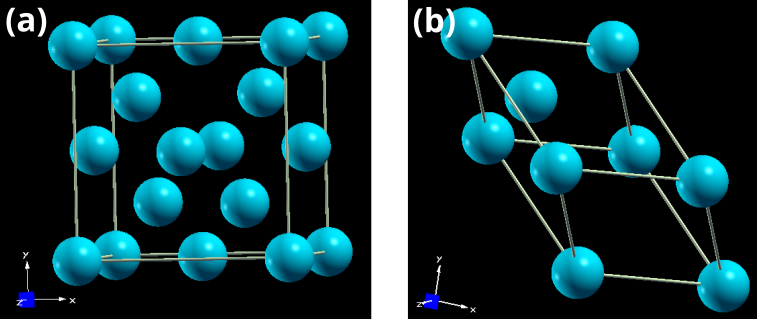
\includegraphics[width = 0.7\textwidth]{figs/ass1_Si_cryst.png}
    \caption{\textbf{(a)} The conventional FCC unit cell with a two atom basis. The lattice constant was found to be 5.43 \AA. with a bond angle of 90$^\circ$. (b) The primitive unit cell obtained from the input file. A lattice constant of 3.8396 {\AA} was found, with a bond angle of 60$^\circ$.}
    \label{fig:ass1_cryst}
  \end{figure}

  \item Visualize LAMMPS simulation 
  
  An overview of the total number of bonds and atoms can for each output file can be found in Table \ref{tab:ass1_lammps-bonds} and \ref{tab:ass1_lammps-atoms}, respectively.
  The types of atoms are clarified by considering a single isolated molecule in Figure \ref{fig:ass1_molecules}. Mainly, Type 1 corresponds to the backbone of the molecule, and Type 2 and 4 correspond to reactive atoms. Further analysis of the \texttt{half\_reacted.data} file showed that Type 3 atoms correspond to reacted Type 2 atoms, see Figure \ref{fig:ass1_molecules}. This reaction is also captured in the introduction of Type 2 bonds, as seen by the number of Type 2 bonds being exactly half of the number of Type 3 atoms. It is important to note, that this suggests that the Type 2 bond is restricted to two atoms. 

  \begin{table}[h]
    \caption{An overview of the number of each bond type for the output files considered.}
    \label{tab:ass1_lammps-bonds}
    \centering
    \begin{tabular}{cccc}
      \hline
    \textbf{Bond Type}      & \textbf{No-reacted}     & \textbf{Half-reacted}   & \textbf{Full-reacted}   \\
    \hline
    1 & 216000 & 216000 & 216000 \\
    2 & 0      & 10947  & 18861  \\
    3 & 0      & 0      & 0      \\
    4 & 0      & 0      & 0      \\ \hline
    \textbf{Total} & 216000 & 226947 & 234861 \\ \hline
    \end{tabular}
  \end{table}

  \begin{table}[h]
    \caption{An overview of the number of each atom type for the output files considered.}
    \label{tab:ass1_lammps-atoms}
    \centering
    \begin{tabular}{cccc}
      \hline
    \textbf{Atom Type}      & \textbf{No-reacted}     & \textbf{Half-reacted}   & \textbf{Full-reacted}   \\
    \hline
    1 & 156000 & 156000 & 156000 \\
    2 & 48000  & 26106  & 10278  \\
    3 & 0      & 21894  & 37722  \\
    4 & 24000  & 24000  & 24000  \\ \hline
    \textbf{Total} & 228000 & 228000 & 228000 \\ \hline
    \end{tabular}
  \end{table}
  
  Using the \texttt{expression selection} feature in \texttt{Ovito} on the \texttt{no\_reaction.data} file, a single, non-bonded, molecule was found to be made up of 19 atoms. Further clustered-by-bonds analysis, Figure \ref{fig:cluster_analysis}, showed that the initial no-reaction configuration consisted of 12000 molecules. This also demonstrates that the system shows no polydispersity as 1200 $\times$ 19 gives the total number of atoms in the system. Similar clustering analysis on the half-reacted system revealed 1418 clusters with the largest consisting of 8123 molecules (154337) atoms while a single molecule was found for the full-reacted system provided by the \texttt{full\_reacted.data} file. 

  Instead of full molecules, the number of new chains formed by the reactions can be considered by first selecting the reacted atoms (Type 3) along with the atom connecting it to the main chain (Type 4) and then performing a similar cluster-by-bonds analysis, Figure \ref{fig:ass1_full_reaction}(a). 
  Such analysis reveals 6424 "clusters", with the largest consisting of 396 atoms. The distribution of the new chain sizes are shown in Figure \ref{fig:ass1_full_reaction}(b).

  \begin{figure}[htbp]
    \centering 
    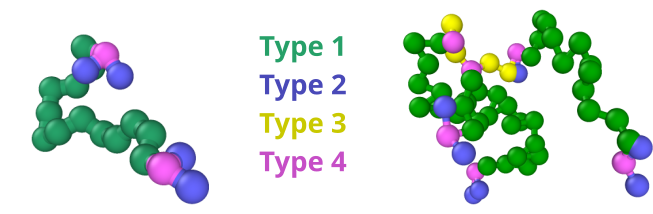
\includegraphics[width = 0.7\textwidth]{figs/ass1_molecules.png}
    \caption{Two isolated molecules demonstrated each atom type. The left shows an isolated molecule extracted from the non-reacted system, while the right was extracted from the half-reacted system.}
    \label{fig:ass1_molecules}
  \end{figure}
  \begin{figure}[htbp]
    \centering 
    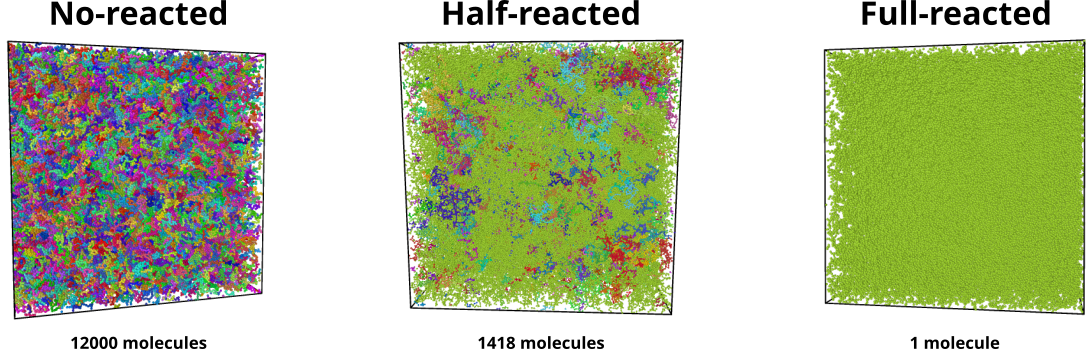
\includegraphics[width = 0.9\textwidth]{figs/ass1_molecule_clusters.png}
    \caption{Clusters of bonded atoms, considered molecules, as determined using \texttt{cluster by bonds} in \texttt{Ovito} on the different systems considered. Different colors represent a different molecule.}
    \label{fig:cluster_analysis}
  \end{figure}
  \begin{figure}[htbp]
    \centering 
    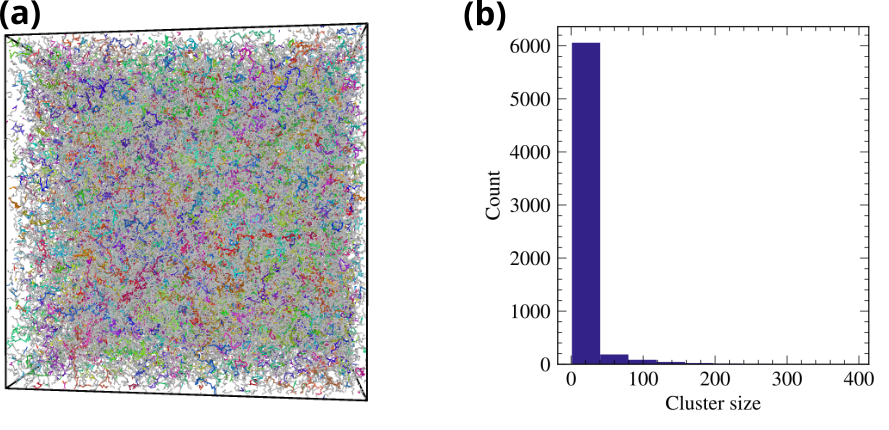
\includegraphics[width = 0.7\textwidth]{figs/ass1_full-reaciton.png}
    \caption{A cluster analysis by bonds for selecting atoms of Type 3 and Type 4. (a) Shows the different clusters (bonds only) with each color representing a separate cluster. (b) Shows the distribution of the cluster sizes using 10 bins. }
    \label{fig:ass1_full_reaction}
  \end{figure}
  
\end{enumerate}

\newpage
\section{Assignment 2: First DFT Simulation}
\begin{enumerate}
  \item Energy Convergence
  
  The final total energy from the original input file with a convergence threshold of \texttt{1d-8}, kinetic energy cutoff of 40 Ry, and 4 k-points in each direction was found to be \texttt{-20.43868608 Ry}.
  This result was achieved after seven iterations as shown in Figure \ref{fig:ass2_conv-thr}(a). The final energy can be more accurate by having a stricter convergence threshold, \texttt{conv\_thr}, which is shown in Figure  \ref{fig:ass2_conv-thr}(b) for \texttt{conv\_thr=1.0d-12}. For the stricter convergence threshold, convergence is achieved after 10 iterations. 

  \begin{figure}[h]
    \centering 
    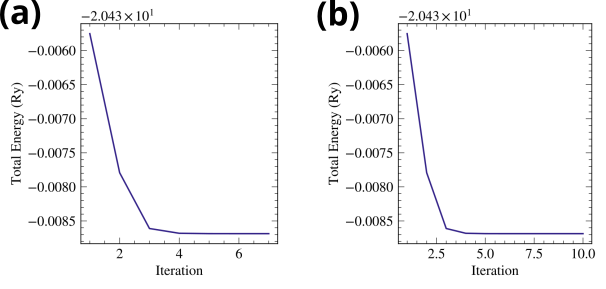
\includegraphics[width = 0.7\textwidth]{figs/ass2_conv-thr.png}
    \caption{The total energy of the simulation as a function of the iteration of the self-consistent field calculation for a convergence threshold of (a) \texttt{1d-8} and (b) \texttt{1d-12}. }
    \label{fig:ass2_conv-thr}
  \end{figure}

  \item Effect of Kinetic energy cutoff \texttt{ecutwfc} and number of k-points \texttt{nk}
  Varying both the kinetic energy cutoff and number of k-points has a significant effect on the accuracy of the final total energy as seen in Figure \ref{fig:ass2_energy-ecut_nks}. 
  Mainly, increasing the number of k-points in each direction from 2 to 8 lead to a 0.01 Ry decrease in the total energy, while increasing \texttt{ecutwfc} from 20.0 Ry to 50.0 Ry lead to a reduction by 0.04 Ry. Therefore, increasing either one leads to a more accurate final energy calculation.   
  
    \begin{figure}[h]
      \centering 
      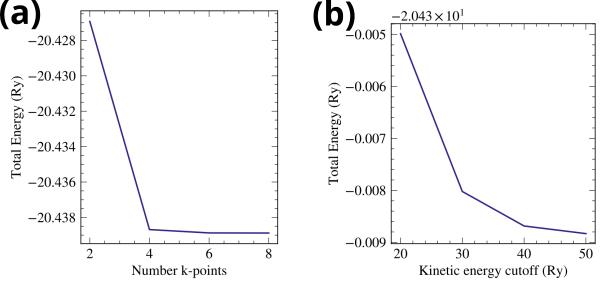
\includegraphics[width = 0.7\textwidth]{figs/ass2_energy-ecut_nks.png}
      \caption{The total energy of the simulation as a function of (a) the number of k-points for \texttt{ecutwfc=40.0} and (b) the kinetic energy cutoff for \texttt{nk=4}. In both cases, the convergence threshold was kept at \texttt{1d-8}.}
      \label{fig:ass2_energy-ecut_nks}
    \end{figure}

\end{enumerate}



\newpage
\section{Assignment 3: First LAMMPS Simulations}

The thermodynamic data for the system ran at a temperature of 1.0 and a packing fraction of 0.45 is shown in Figure \ref{fig:ass3_thermo}. As all parameters are relatively stable over the simulation, it can be said that the system is in equilibrium. 

\begin{figure}[htpb]
  \centering 
  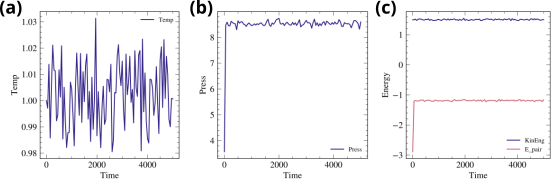
\includegraphics[width = 0.9\textwidth]{figs/ass3_thermo.png}
  \caption{The thermodynamic data over time as extracted from the \texttt{log.lammps} file for a system at temperature $T=1.0$ and packing fraction \texttt{eta=0.45}. (a) is the temperature of the system, (b) the pressure of the system, and (c) the Kinetic and potential energy of the system.}
  \label{fig:ass3_thermo}
\end{figure}

The effect of different temperatures and packing fractions on the structure and dynamics of the system are demonstrated in Figures \ref{fig:ass3_struc} and \ref{fig:ass3_rdf-msd}. 
The structural visualization using the \texttt{Common neighbor} analysis in \texttt{Ovito}, Figure \ref{fig:ass3_struc} suggests that for a packing fraction of 0.45, there is no crystalization and that the systems are liquid. This is supported by the RDFs of these systems, Fig \ref{fig:ass3_rdf-msd}(a), demonstrating a large peak at $r/\sigma = 1$ followed by smaller decaying peaks. However, it is noted that the MSD of T0.5-eta0.45, Figure \ref{fig:ass3_rdf-msd}(b) shows an inflection point and short plateau starting at $\tau\approx 1.0$, followed by a super diffusive regime, which is characteristic of glassy/caging dynamics.  

Additionally, for packing fractions of 0.6 and 0.7 at temperature 1.0 show crystal domains mainly of HCP and FCC structure. This is also supported by the sharp peaks observed in the corresponding RDFs, Figure \ref{fig:ass3_rdf-msd}(c). Moreover, both MSDs for eta=0.6,0.7, Figure \ref{fig:ass3_rdf-msd}(d) show a strong plateau after the ballistic regime, which is indicative of a solid like material. 

\begin{figure}[htpb]
  \centering 
  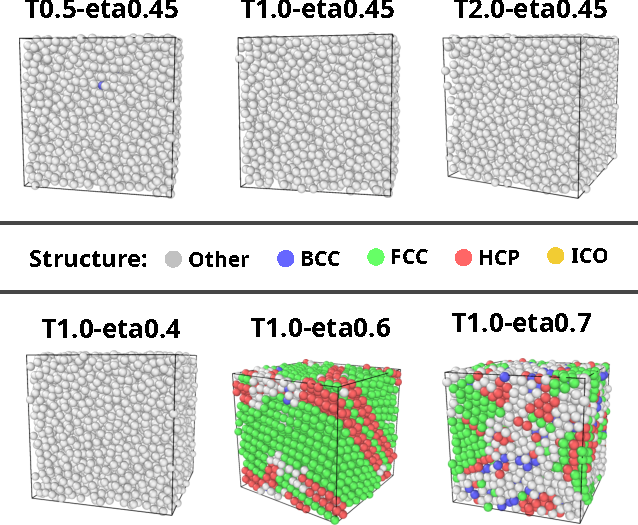
\includegraphics[width = 0.6\textwidth]{figs/ass3_struct.pdf}
  \caption{Visualizations of the varied parameters for the simple LAMMPS system. (Top) Varying the temperature $T$ for a constant packing fraction \texttt{eta}. (Middle) The color scheme for the structure offered by the \texttt{Common neighbor} analysis in \texttt{Ovito}. (Bottom) Various packing fractions for a constant temperature $T$. }
  \label{fig:ass3_struc}
\end{figure}
\begin{figure}[htpb]
  \centering 
  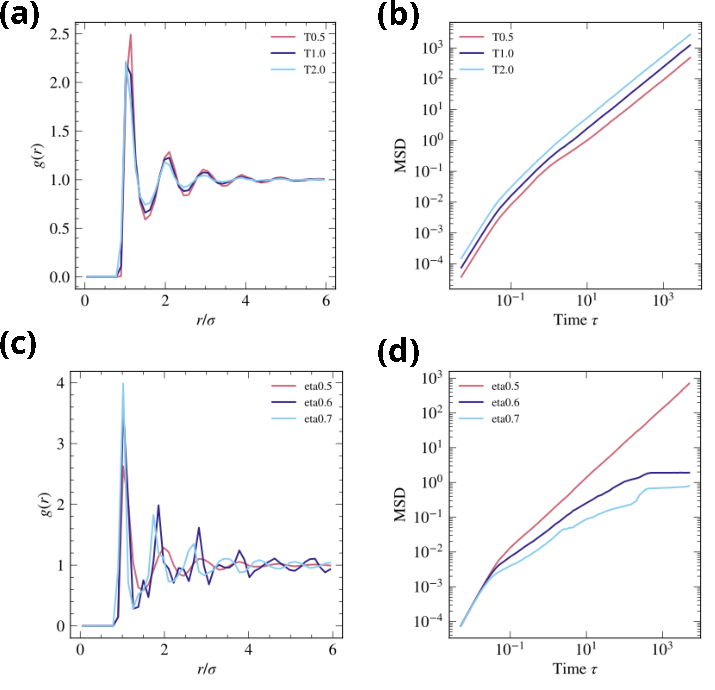
\includegraphics[width = 0.8\textwidth]{figs/ass3_rdf-msd.pdf}
  \caption{The RDF and MSD for the samples in Figure \ref{fig:ass3_struc}. (a-b) correspond to a fixed packing fraction of 0.45 while (c-d) correspond to a fixed temperature of 1.0. For the fixed packing fraction, all systems show a liquid characteristic, with glassy behavior emerging at T=0.5. Increasing packing fraction leads to a crystal grains, with more regular packing showing for a packing fraction of 0.6. }
  \label{fig:ass3_rdf-msd}
\end{figure}

\section{Assignment 4: Benchmarking}

\begin{enumerate}
  \item Benchmarking Quantum Espresso DFT calculation
  
  \begin{table}[h]
    \caption{An overview of the total wall time in seconds for different number of processors used on the parallel partition on Habrok for 4 and 16 k-points (nk). For each simulation \texttt{ecutwfc=40.0 Ry}, \texttt{conv\_thr=1d-8} was used. Each simulation provided the same lattice constant as mentioned in Figure \ref{fig:ass1_cryst}(b), within the limit provided by \texttt{xcrysden}. From Figure \ref{fig:ass2_energy-ecut_nks}(a), the accuracy in final energy increased the most when moving to \texttt{nk=4}, thus, extra parallelization here is not optimal: the calculation using 12 processors and \texttt{nk=4} is most optimal. }
    \label{tab:ass4_DFT-benchmark}
    \centering
    \begin{tabular}{c|ccc}
      \hline
      \multirow{2}{*}{nk} & \multicolumn{3}{c}{Number Processors} \\
                          & 2           & 12         & 64         \\ \hline
      4                   & 0.89        & 0.63       & 0.53       \\
      16                  & 17.34       & 9.93       & 2.90       \\ \hline
      \end{tabular}
  \end{table}

\item Benchmarking LAMMPS MD Simulations

\begin{table}[htbp]
  \caption{The performance of the LAMMPS simulation of 4096 particles with one task per node for increasing cut-off distances of the LJ potential.}
  \label{tab:ass4_lammps-lj}
  \centering
  \begin{tabular}{cc} \hline
    \textbf{\texttt{lj\_cut}} $\bm{\sigma}$ & \textbf{Performance (steps/s)}\\
    \hline
    1.12                        & 1260.628                        \\
    2.0                         & 450.479                         \\
    4.0                         & 90.332                          \\
    6.0                         & 32.678                          \\ \hline
    \end{tabular}
\end{table}

\begin{table}[htbp]
  \caption{The performance of the LAMMPS simulation of 4096 particles with one task per node for increasing cut-off distances of the \texttt{lj/cut/coul/cut} potential. \texttt{lj\_cut} was kept at 1.12 $\sigma$. Each particle had a charge of +1.}
  \label{tab:ass4_lammps-coul}
  \centering
  \begin{tabular}{cc} \hline
    \textbf{\texttt{coul\_cut}} $\bm{\sigma}$ & \textbf{Performance (steps/s)}\\
    \hline
    1.12                        & 1226.768                        \\
    2.0                         & 398.870                        \\
    4.0                         & 80.435                          \\
    6.0                         & 29.116                          \\ \hline
    \end{tabular}
\end{table}

\begin{table}[htb]
  \caption{The performance of the LAMMPS simulation of $N$ particles with one task per node for \texttt{lj/cut} interactions with a cut-off distances of 1.12 $\sigma$ and \texttt{lj/cut/coul/cut} interactions with cut-off distances of 1.12 and 6.0 $\sigma$. For the \texttt{lj/cut/coul/cut} interactions, each particle had a charge of +1.}
  \label{tab:ass4_lammps-npart}
  \centering
  \begin{tabular}{ccc} \hline
    \textbf{\texttt{N}} & \textbf{steps/s (lj/cut) }& \textbf{steps/s (lj/cut/coul/cut)}\\
    \hline
    4096                        & 1260.628      &       29.116           \\
    8192                         & 627.877       &      14.173           \\
    12288                         & 419.067      &      9.787              \\
    16384                         & 297.377       &     7.012              \\ \hline
    \end{tabular}
\end{table}

\begin{table}[htb]
  \caption{The performance of the LAMMPS simulation of 4096 particles with $M$ tasks per node (processors) for \texttt{lj/cut} interactions with a cut-off distances of 1.12 $\sigma$ and \texttt{lj/cut/coul/cut} interactions with cut-off distances of 1.12 and 6.0 $\sigma$. For the \texttt{lj/cut/coul/cut} interactions, each particle had a charge of +1. 
  Comparing the performance values to those obtained in the first row of Table \ref{tab:ass4_lammps-lj} and last row of Table \ref{tab:ass4_lammps-coul}, shows that parallelization of LAMMPS on Habrok can lead to substantial increases in efficiency.}
  \label{tab:ass4_lammps-nproc}
  \centering
  \begin{tabular}{ccc} \hline
    \textbf{\texttt{M}} & \textbf{steps/s (lj/cut) }& \textbf{steps/s (lj/cut/coul/cut)}\\
    \hline
    2                        & 2449.352      &       57.569          \\
    4                         & 4124.183       &      111.287           \\
    8                         & 6796.371      &      196.499              \\
    16                         & 10838.676      &     417.952              \\ 
    32                        &  9851.291        &  604.731\\ \hline
    \end{tabular}
\end{table}
\end{enumerate}

\newpage
% \printbibliography

% \begin{appendices}
%   \input{Appendix}
% \end{appendices}

\end{document}



